\section{Formattazione di base}
\subsection{Effetti sul testo}
\begin{frame}
 \frametitle{Formattazione di base}
 
 Come su altri elaboratori di testo è presente:
 \begin{itemize}
  \item<1-> Il \textit{corsivo} con \texttt{\textbackslash textit}
  \item<2-> Il \textbf{grassetto} con \texttt{\textbackslash textbf}
  \item<3-> Il \underline{sottolineato} con \texttt{\textbackslash underline}
  \item<4-> Lo \sout{sbarrato} con \texttt{\textbackslash sout}
  \begin{itemize}
   \item Bisogna usare il pacchetto \texttt{ulem}
  \end{itemize}

 \end{itemize}
 
 \begin{textblock*}{5cm}(7.5cm,4cm)
   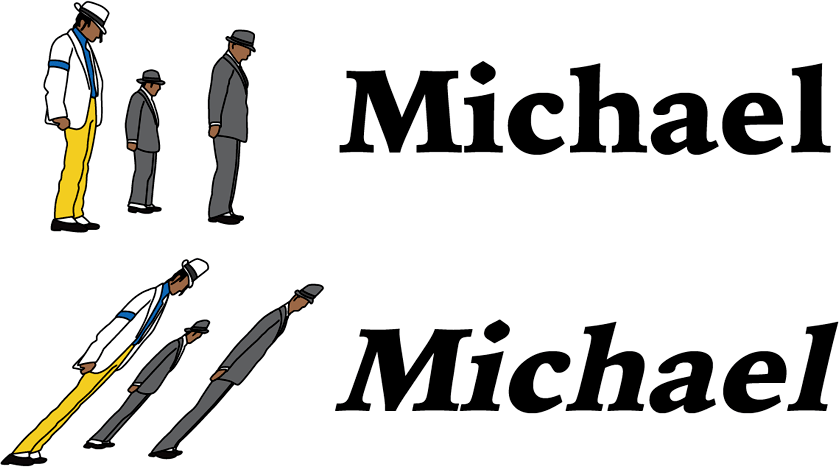
\includegraphics[scale=0.15]{jacksons}
 \end{textblock*}
\end{frame}
